\documentclass[t, aspectratio=169]{beamer}
\usepackage{amsmath,amsfonts,amsthm,amstext,amssymb, xcolor, tikz, pgf, mathrsfs, polynom, pifont, tabto}

% ----------------------------------------------------------
% Theme Setup

% Use Metropolis Theme
\usetheme[numbering=fraction]{metropolis}
\setbeamertemplate{blocks}[rounded][shadow=false]
\makeatletter
\setlength{\metropolis@titleseparator@linewidth}{1pt}
\makeatother

% Define Colors
\definecolor{chargerblue}{HTML}{002764}
\definecolor{chargerred}{HTML}{e02034}
\definecolor{bggray}{HTML}{d0d3d4}

% Set Colors
\setbeamercolor{title}{fg=chargerblue}
\setbeamercolor{background canvas}{bg=white}
\setbeamercolor{title separator}{fg=chargerred}
\setbeamercolor{structure}{fg=chargerblue}
\setbeamercolor{frametitle}{fg=white, bg=chargerblue}
\setbeamercolor*{normal text}{fg=chargerblue}
\setbeamercolor*{block body}{bg=bggray}
\setbeamercolor*{block title}{bg=chargerblue, fg=white}
% ----------------------------------------------------------

% ----------------------------------------------------------
% Custom Definitions, Commands, Environments, etc.

% Sets of numbers
\def\R{\mathbb{R}} % The reals
\def\N{\mathbb{N}} % The naturals
\def\Z{\mathbb{Z}} % The integers
\def\Q{\mathbb{Q}} % The rationals

% Blank space
\newcommand{\blank}[1]{\underline{\hspace{#1}}} % Blank space

% Change font colors
\newcommand{\cyan}[1]{{\color{cyan}{#1}}} % Changes font to cyan
\newcommand{\red}[1]{{\color{red}{#1}}} % Changes font to red
\newcommand{\magenta}[1]{{\color{magenta}{#1}}} % Changes font to magenta
\newcommand{\orange}[1]{{\color{orange}{#1}}} % Changes font to orange
\newcommand{\yellow}[1]{{\color{yellow}{#1}}} % Changes font to yellow
\newcommand{\violet}[1]{{\color{violet}{#1}}} % Changes font to violet
\newcommand{\green}[1]{{\color{green}{#1}}} % Changes font to green
\newcommand{\blue}[1]{{\color{blue}{#1}}} % Changes font to blue
\newcommand{\white}[1]{{\color{white}{#1}}} % Changes font to white

% Fitted inclusion symbols
\newcommand{\fp}[1]{\left({#1}\right)} % Fitted parentheses around content
\newcommand{\fb}[1]{\left[{#1}\right]} % Fitted brackets
\newcommand{\lhoi}[1]{\left({#1}\right]} % Left half-open interval
\newcommand{\rhoi}[1]{\left[{#1}\right)} % Right half-open interval
\newcommand{\set}[1]{\left\{{#1}\right\}} % Fitted braces (useful for sets)
\newcommand{\av}[1]{\left|{#1}\right|} % Fitted absolute value bars

% Augmented Matrix Environment
\newenvironment{amatrix}[1]{%
	\left[\begin{array}{@{}*{#1}{c}|c@{}}
	}{%
	\end{array}\right]
}

% Miscellaneous
\def\then{\Rightarrow}
\def\to{\rightarrow}
\def\d{^{\circ}}
\newcommand{\?}{\stackrel{?}{=}}
\newcommand{\cmark}{\text{ \ding{51}}}
\newcommand{\xmark}{\text{ \ding{55}}}

% Coordinate Plane (Four-Quadrant)
\def\coordplane {
	\begin{tikzpicture}        \draw[step=0.25cm,black,very thin,opacity=0.25] (-2.5cm, -2.5cm) grid (2.5cm, 2.5cm);
		\draw[<->,thick,black] (-2.5cm, 0) -- (2.5cm, 0) node[anchor=north west,pos=0.94,font=\scriptsize]{$x$};
		\draw[<->,thick,black] (0,-2.5cm) -- (0, 2.5cm) node[anchor=south east,font=\scriptsize,pos=0.94]{$y$};
	\end{tikzpicture}
}

% Coordinate Plane (One-Quadrant)
\def\onequad {
	\begin{tikzpicture}
		\draw[step=0.25cm, black, very thin, opacity=0.25] (0,0) grid (7.5cm,5cm);
		\draw[->, thick, black] (0,0) -- (7.5cm, 0) node[anchor=north west,font=\scriptsize,pos=0.94]{$x$};
		\draw[->, black, thick] (0,0) -- (0,5cm) node[anchor=south east,font=\scriptsize,pos=0.94]{$y$};
	\end{tikzpicture}
}
% ----------------------------------------------------------

% ----------------------------------------------------------
% Presentation Information
\title[4-1]{Sample Spaces and Probability}
\subtitle{Section 4-1}
\author{Jacob Ayers}
\institute{Lesson \#9}
\date{MAT 110}
% ----------------------------------------------------------

\begin{document}
	
	% Slide 1 (Title Slide)
	\begin{frame}
		\titlepage
	\end{frame}
	
	% Slide 2 (Objectives)
	\begin{frame}{Objectives}
		\begin{itemize}
			\item Determine the sample space of an experiment
			\item Find the probability of an event occurring
			\item Understand the difference between classical probability and empirical probability
		\end{itemize}
	\end{frame}

	\begin{frame}{Basic Concepts}
		\textit{Probability experiment}: chance process leading to well-defined results called \textit{outcomes} \pause
		
		\textit{Outcome}: result of single trial of a probability experiment \pause
		
		Examples: Flipping a coin, drawing a card from a deck, rolling a die
	\end{frame}

	\begin{frame}{Sample Space of a Probability Experiment}
		The \textit{sample space} of a probability experiment is the set of all possible outcomes for the experiment. \pause
		
		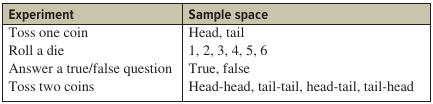
\includegraphics[width=4in]{ss-ex.png}
	\end{frame}

	\begin{frame}{Sample Space of a Probability Experiment}
		There are a few different methods that we can use to find the sample space of a probability experiment: \begin{itemize}
			\item Observation/reasoning
			\item Create a table
			\item Create a tree diagram
		\end{itemize} \pause
	
		Example: Find the sample space for the gender of the children if a family has two children. \pause
		
		Here, we can reason our way through the possibilities pretty easily. \pause They are: \\
		BB, BG, GB, GG
	\end{frame}

	\begin{frame}{Sample Space of a Probability Experiment}
		Find the sample space of rolling two six-sided dice. \pause
		
		A table will be useful here. \pause
		
		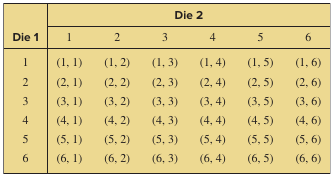
\includegraphics[width=4in]{two-dice.png}
	\end{frame}

	\begin{frame}{Sample Space of a Probability Experiment}
		Find the sample space of flipping a fair coin three times. \pause
		
		I'll use a tree diagram to find all the outcomes this time.
	\end{frame}

	\begin{frame}{Classical Probability}
		We often need to find the probability of two or more outcomes.
		
		An \textit{event} is a set of outcomes of a probability experiment. \pause
		
		Examples of events: rolling a 6 (simple event), drawing a spade from a deck of cards (compound event) \pause
		
		\textit{Probability of an event}: likelihood that an event will occur. \pause
		
		Examples: \\ Probability of rolling a 6: $\dfrac16$ \\ Probability of getting heads on coin toss: $\dfrac12$
	\end{frame}

	\begin{frame}{Classical Probability}
		\textit{Classical probability} uses sample spaces to determine probability - it is based on theory, not on results of experiments. \pause
		
		Key assumption: All outcomes in the sample space are equally likely to occur (i.e. have the same probability) \pause
		
		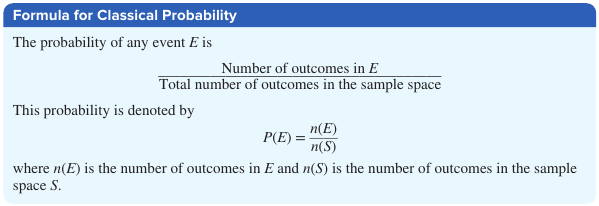
\includegraphics[width=5in]{classical.png}
	\end{frame}

	\begin{frame}{Classical Probability}
		If a family has three children, find the probability that exactly two of them will be girls. \pause
		
		First, we need to write out the sample space. \\
		BBB, BBG, BGB, BGG, GBB, GBG, GGB, GGG \pause
		
		There are a total of eight outcomes, and three of them involve having exactly two girls. \pause
		
		Therefore, $P(\text{exactly two girls}) = \dfrac38$
	\end{frame}

	\begin{frame}{Classical Probability}
		The next several examples will involve drawing cards from a 52-card deck. \pause
		
		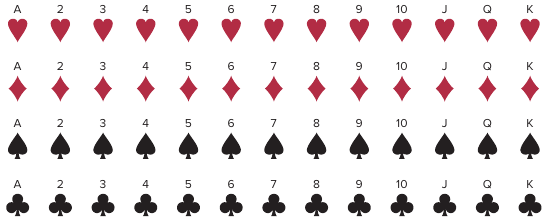
\includegraphics[width=4in]{deck-cards.png}
	\end{frame}

	\begin{frame}{Classical Probability}
		A card is drawn from a 52-card deck. Find the probability of getting: \begin{enumerate}[a)]
			\item A heart
			\item A black card
			\item The 8 of diamonds
			\item A face card
		\end{enumerate} \pause
		\begin{enumerate}[a)]
			\item There are 13 hearts. So $P(\heartsuit) = \dfrac{13}{52} = \dfrac14$ \pause
			\item There are 26 black cards. So $P(\text{black}) = \dfrac{26}{52} = \dfrac12$ \pause
			\item There is just one 8 of diamonds. So $P(8\diamondsuit) = \dfrac{1}{52}$ \pause
			\item There are 12 face cards. So $P(\text{face}) = \dfrac{12}{52} = \dfrac{3}{13}$
		\end{enumerate}
	\end{frame}

	\begin{frame}{Probability Rules}
		Rounding rule: If expressing probability as a decimal, round to three decimal places. \pause
		
		The probability of any event $E$ is between 0 and 1 (inclusive). Mathematically: $0 \leq P(E) \leq 1$ \pause
		
		The sum of the probabilities of all the outcomes in the sample space is $1$.
		
		If an event cannot occur, then $P(E) = 0$. \pause
		
		If an event is certain to occur, then $P(E) = 1$.
	\end{frame}

	\begin{frame}{Complementary Events}
		The \textit{complement of an event} $E$ is the set of outcomes that are not in $E$.
		
		Notation: $\overline{E}$ denotes the complement of $E$. \pause
		
		Example: Find the complement of each event: \begin{enumerate}[a)]
			\item Selecting a month that has 31 days.
			\item Selecting a card that is an ace.
		\end{enumerate} \pause
		\begin{enumerate}[a)]
			\item Selecting a month that doesn't have 31 days (Feb., Apr., June, Sept., Nov.) \pause
			\item Selecting a card that is not an ace (2, 3, 4, 5, 6, 7, 8, 9, 10, J, Q, K)
		\end{enumerate}
	\end{frame}

	\begin{frame}{Empirical Probability}
		\textit{Empirical probability} is probability that relies on past results. It \textit{doesn't} assume that all outcomes in the sample space are equally likely. \pause
		
		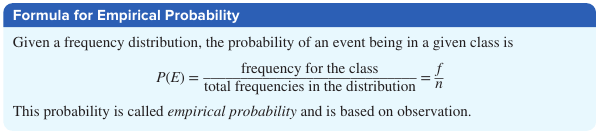
\includegraphics[width=\textwidth]{empirical.png}
	\end{frame}

	\begin{frame}{Empirical Probability}
		The following information shows the amount of debt students who graduated from college incur for a specific year.
		
		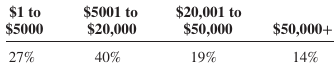
\includegraphics[width=3in]{college-debt.png}
		
		If a person who graduates has some debt, find the probability that \begin{enumerate}[a)]
			\item It is less than \$5001. \pause 27\% or $0.27$
			\item It is more than \$20000. \pause 33\% or $0.33$
			\item It is between \$1 and \$20000. \pause 67\% or $0.67$
		\end{enumerate}
	\end{frame}

	\begin{frame}{Empirical Probability}
		During a recent year, there were 13.5 million automobile accidents, 5.2 million truck accidents, and 178,000 motorcycle accidents. If one accident is selected at random, find the probability that it was not a car accident. \pause
		
		\underline{Method 1: Using the Complement} \\
		First, find the probability that it was a car accident: $P(\text{car}) = \dfrac{13,500,000}{18,878,000} \approx 0.715$. \pause
		
		So $P(\text{not car}) = 1 - P(\text{car}) \approx 1 - 0.715 \approx 0.285$. \pause
		
		\underline{Method 2: Compute Directly} \\
		If the accident wasn't a car accident, it was a truck or motorcycle accident.
		
		$P(\text{not car}) = \dfrac{5,200,000 + 178,000}{18,878,000} \approx 0.285$
	\end{frame}

	\begin{frame}{Law of Large Numbers}
		Results of experiments will not always line up with the classical probability.
		
		Example: If I roll a die 6 times, am I guaranteed to get a 1, a 2, a 3, a 4, a 5, and a 6? \pause \\
		No. As a matter of fact, this outcome is pretty unlikely (about 1.54\%)
		
		But if I roll a die 6,000,000 times, I will likely get about 1,000,000 of each outcome. \pause
		
		This is the law of large numbers at work. \pause
		
		The \textit{law of large numbers} states that as the number of trials of an experiment increases, the empirical probability will approach the theoretical probability.
	\end{frame}

	\begin{frame}{Next Steps}
		\begin{itemize}
			\item Read 4-2
			\item Watch Video Lesson \#10
		\end{itemize}
	
		\vfill
		
		Thanks for watching!
	\end{frame}
	
\end{document}